%% ICDE 2027 Round 2, EAB. <=12 pages excl. references and AI acknowledgement.
\documentclass[conference]{IEEEtran}
\IEEEoverridecommandlockouts
\usepackage{cite}
\usepackage{amsmath,amssymb}
\usepackage{graphicx}
\usepackage{booktabs}
\usepackage{array}
\usepackage{colortbl}
\newcommand{\rowsep}{\arrayrulecolor{black!20}\specialrule{0.3pt}{1.5pt}{1.5pt}\arrayrulecolor{black}}
\usepackage{xcolor}
\usepackage{listings}
\usepackage{url}
\usepackage{tikz}
\usepackage{algorithm}
\usepackage{algpseudocode}
\usetikzlibrary{positioning,arrows.meta,fit}
\usepackage[hidelinks]{hyperref}
\lstset{basicstyle=\ttfamily\footnotesize, breaklines=true, columns=fullflexible,
        frame=single, framerule=0.3pt, xleftmargin=2pt, xrightmargin=2pt,
        aboveskip=3pt, belowskip=3pt}
\newcommand{\todo}[1]{\textcolor{red}{[TODO: #1]}}
\newcommand{\sys}{\textsc{GoldCheck}}
\newtheorem{definition}{Definition}

\begin{document}

\title{[Experiment, Analysis, and Benchmark] Right by Accident: Text-to-SQL Gold Queries Whose Answers Depend on the Database State}

\author{%
\IEEEauthorblockN{Jiacheng Ding\textsuperscript{1}, Cong Guo\textsuperscript{1}, Peihua Mai\textsuperscript{2,*}}
\IEEEauthorblockA{\textsuperscript{1}University of Memphis, Memphis, TN, USA\\
\textsuperscript{2}National University of Singapore, Singapore\\
jding2@memphis.edu, cguo@memphis.edu, peihua.m@u.nus.edu}
\thanks{\textsuperscript{*}Corresponding author.}
}

\maketitle

\begin{abstract}
Text-to-SQL benchmarks score a system by running its query and a reference
query, the gold query, on one database and comparing the results. Each gold
query is therefore checked against a single database state. We study gold
queries whose answer depends on that state in a way the question does not
intend. Some cut a ranked list at a tie and return whichever tied row the engine
produces first. Some count join rows where the question asks for entities. Some
return nothing, so the benchmark accepts any prediction that also matches
nothing. We define such \emph{state-dependent} gold queries and present \sys{},
a deterministic checker that reports a finding only with a proof by execution.
The proof is a second reading of the query that disagrees with the gold on the
official database, or a one-cell edit of the database on which the two readings
disagree. In three independent human reviews of the BIRD gold, the review
changed the output of flagged queries 2.3 to 4.1 times as often as the output of
other queries. On 1,036 examples that we never inspected, the ratio is 2.4, with
a 95\% interval from 1.7 to 3.3. Static SQL rules and one-time execution reach
at most 1.7. The latest official BIRD Dev release still contains 65 flagged
queries. For 31 of them, the test is defective whatever the question intends,
and two annotators independently judged 26 of the other 34 to be errors. \sys{}
needs a median of 17\,ms per query and no language model. Rebuilding the tables
without changing the data changes the gold answer of 12 of the 21 tie queries.
An LLM reviewer names more count fan-outs as it grows from 3B to 120B
parameters, but it names at most 11 of 41 ties unless it receives the evidence
from \sys{}.
\end{abstract}

\begin{IEEEkeywords}
text-to-SQL, benchmarks, data quality, query testing, test data generation
\end{IEEEkeywords}

\section{Introduction}

Large language models (LLMs) have renewed interest in how people and programs
talk to databases. Text-to-SQL translates a question into an executable query.
It is the most direct form of this interaction, and both the database and the
language communities now build and compare such
systems~\cite{li2024dawn,floratou2024nl2sql,lei2025spider2}. Researchers measure
progress on benchmarks such as BIRD~\cite{li2024bird} and
Spider~\cite{yu2018spider}. Each example pairs a question with a database and a
reference query, the \emph{gold} query. A benchmark scores a system's query as
correct when it returns the same result as the gold query on the benchmark
database. Leaderboard numbers therefore rest on the gold queries.

People write gold queries, and people make errors. A recent audit found errors
in more than half of the examples of BIRD Mini-Dev and Spider~2.0-Snow and
showed that corrections reorder a leaderboard~\cite{jin2026pervasive}. The BIRD
maintainers released a reviewed Dev set in November 2025~\cite{bird2025dev}.
These reviews are expensive. The audit used an LLM agent, SAR-Agent, that costs
\$0.44 per example with OpenAI o3, and two authors checked every report it
produced~\cite{jin2026pervasive}. Five researchers led the maintainers' review
with a larger group of reviewers~\cite{bird2025dev}.

This paper studies one kind of gold error that is easy to make, hard to see,
and cheap to find automatically. An annotator writes a gold query and checks it
on one database. If it returns a plausible answer there, the annotator accepts
it. But a query can return the expected answer on that one database by accident.
Fig.~\ref{fig:examples} shows three gold queries from the latest official BIRD
Dev release.
\begin{itemize}
\item \emph{``Who is the tallest superhero?''} The gold query sorts by height and
keeps one row. Two superheroes, Surtur and Ymir, share the largest height of
30,480\,cm. The gold answer is Surtur because SQLite happens to return that row
first. A system that lists both receives no credit.
\item \emph{``How many female patients have a white blood cell count below
3.5?''} The gold query joins patients to lab tests and counts patient
identifiers without \texttt{DISTINCT}. It returns 641, the number of lab tests.
The number of patients is 88.
\item \emph{``What is the average total price of the transactions in January
2012?''} The database has no such transactions. The gold answer is
\texttt{NULL}, the value an average takes over no rows. A system whose query
also matches no rows receives full credit, for example a query that filters on a
wrong date format.
\end{itemize}
In each case, running the gold query raises no flag. It returns one plausible
value. The problem lies in how the answer depends on the data.

\begin{figure}[t]
\small
\textbf{(a) Tie at the cut.} \emph{Who is the tallest superhero?}
\begin{lstlisting}
SELECT superhero_name FROM superhero
ORDER BY height_cm DESC LIMIT 1        -- Surtur
-- Ymir has the same height and is cut off
\end{lstlisting}
\textbf{(b) Count fan-out.} \emph{How many female patients have a white
blood cell count below 3.5?}
\begin{lstlisting}
SELECT COUNT(T1.ID)
FROM Patient T1 JOIN Laboratory T2 ON T1.ID = T2.ID
WHERE T2.WBC < 3.5 AND T1.SEX = 'F'
-- 641; COUNT(DISTINCT T1.ID) is 88
\end{lstlisting}
\textbf{(c) Empty answer.} \emph{What is the average total price of the
transactions in January 2012?}
\begin{lstlisting}
SELECT AVG(Price) FROM transactions_1k
WHERE Date LIKE '2012-01%'             -- NULL
\end{lstlisting}
\caption{Three gold queries from the 2025-11-06 BIRD Dev release, lightly
abridged. Comments show what \sys{} reports.}
\label{fig:examples}
\end{figure}

We call such queries \emph{state-dependent}. The database community has long
known that one database state is a weak test of a query. Test data generation
for SQL grading~\cite{chandra2015xdata}, test suites for text-to-SQL
predictions~\cite{zhong2020test}, and database-engine
testing~\cite{rigger2020pqs,rigger2020tlp} all vary the state. The gold query is
the oracle for everything else, yet benchmarks still check it on one state. Jin
et al.\ noticed this in passing and hand-inserted distinguishing rows for 6 of
the 100 Dev examples they corrected~\cite{jin2026pervasive}. We turn that
observation into a systematic check.

\textbf{Approach.} \sys{} targets three SQL constructs whose meaning depends on
the data. They are a ranked list cut by \texttt{LIMIT}, a count over a join, and
an empty answer. For each construct, \sys{} builds a second reading of the gold
query and runs both readings on the official database. It reports a finding only
when it can show a concrete difference. When the official data happen not to
separate the readings, it edits one cell to produce a state that does. Every
finding comes with an executable witness. A person still decides whether the
finding is an error, because only the question says which reading it intends.

\sys{} is small. It uses no language model, gives the same answer on every run,
and checks the 1,534 BIRD Dev queries in about a minute. Our goal is to measure
how far a benchmark can trust a single database state as a test, and to provide
a check that makes the gap visible before a person or an LLM agent spends effort
on a review.

\textbf{Contributions.} This paper makes four contributions.
\begin{itemize}
\item[(1)] \textbf{Problem.} We define state-dependent gold queries. A
\emph{live} finding is visible on the official database, and a \emph{latent}
finding needs a one-cell change.
\item[(2)] \textbf{Checker.} \sys{} detects four classes of live findings and
synthesizes one-cell witnesses for latent ones. It proves each finding by
execution, with a median cost of 17\,ms per query.
\item[(3)] \textbf{Comparison with human reviews and baselines.} In three
independent reviews of the BIRD gold, the review changed the output of 35\% to
57\% of flagged queries, 2.3 to 4.1 times the rate of other queries. Static
rules and one-time execution reach at most 1.7.
\item[(4)] \textbf{Evidence that the cause is the test design.} Rebuilding the
tables of the latest release without changing the data changes 12 of its 21 tie
answers. SAR-Agent on open models from 3B to 120B parameters names at most 11 of
41 ties, and 27 to 37 once it receives the evidence from \sys{}.
\end{itemize}
We also report three case studies, on predictions of four open models, on the
BIRD training split, and on a prior ranking analysis. We release \sys{}, the
aligned corpus, and every script behind each number at
\url{https://github.com/graphuofm/goldcheck}.

\section{Preliminaries and Related Work}
\label{sec:prelim}

\subsection{Execution-based scoring}
BIRD~\cite{li2024bird} has questions over 95 databases. Its Dev split has 1,534
questions over 11 SQLite~\cite{gaffney2022sqlite} databases from domains such as
schools, banking, medicine, motorsport, and card games. Each example has a
question, an optional \emph{evidence} note with a domain convention, a gold
query, and a difficulty label. BIRD scores a prediction $P$ by execution match
on the official database $D$. It counts $P$ as correct if and only if the result
\emph{sets} of $P(D)$ and $G(D)$ are equal, where $G$ is the gold query.
Mini-Dev is a 500-example subset of Dev.

\subsection{State-dependent gold queries}
\label{sec:problem}
Let $q$ be a question, $D$ the official database, and $G$ the gold query.
Execution match compares a prediction with $G(D)$ and nothing else. The test is
only as good as the pair $(G, D)$. If what $q$ asks does not determine $G(D)$,
or if $G(D)$ cannot separate a right prediction from a wrong one, the test fails
silently.

Some SQL constructs admit more than one reasonable reading. One row or every
row with the largest height can answer ``the tallest superhero''. A count of rows
or a count of distinct patients can answer ``how many patients''. We write $G_c$
for the gold query with construct $c$ replaced by its other reading.

\begin{definition}[Live finding]
$G$ has a live finding on $D$ if (i) $G(D) \neq G_c(D)$ for some construct
$c$, (ii) $G$ cuts a ranked list and the first ranked row has a \texttt{NULL}
sort key, or (iii) $G(D)$ is empty or contains only \texttt{NULL} values.
\end{definition}

\emph{Example.} For the tallest superhero in Fig.~\ref{fig:examples}(a), $G(D)$
is $\{\text{Surtur}\}$ and the tie-complete reading $G_c(D)$ is
$\{\text{Surtur}, \text{Ymir}\}$. This is a live finding of case (i). The query
in Fig.~\ref{fig:examples}(c) returns only \texttt{NULL} and is a live finding
of case (iii).

\begin{definition}[Latent finding]
$G$ has a latent finding on $D$ if $G(D) = G_c(D)$ but there is a database $D'$
that differs from $D$ in a single cell such that $G(D') \neq G_c(D')$.
\end{definition}

\emph{Example.} A gold query returns the phone number of the school with the
most test takers. On $D$, one school has the largest count, so $G(D) = G_c(D)$.
If the count of a second school is set to the same value, $G$ returns one phone
number and $G_c$ returns two.

\textbf{Terms.} We use four terms with one meaning each. A \emph{finding} is a
live or latent finding as defined above. A \emph{flagged query} is a gold query
with at least one live finding. A \emph{defective test} is a flagged query whose
test fails whatever the question intends, which holds for ties and empty
answers. An \emph{error} is a flagged query that a person judged wrong from the
question. A finding proves that two readings differ on a concrete database. It
does not prove an error, because only the question says which reading it
intends.

\textbf{Role of the engine.} The live cases fail in different ways. (1)
\emph{Ties.} The SQL standard leaves the order of rows with equal sort keys to
the implementation. A query with \texttt{ORDER BY $o$ LIMIT $k$} does not define
its result when the $k$-th and $(k{+}1)$-th rows share the value of $o$. The
engine returns whichever tied row it meets first. (2) \emph{\texttt{NULL} at the
top.} Engines disagree on where \texttt{NULL} sorts. SQLite and MySQL place it
before every other value in ascending order, and PostgreSQL places it after. (3)
\emph{Fan-out and empty answers.} These are deterministic. A count over a join
returns the number of join rows. It equals the number of entities only when no
entity matches more than one row. An empty answer makes the test vacuous, since
the gold agrees with any query that also matches nothing.

\textbf{Scope.} We chose the classes from the research audit of
Mini-Dev~\cite{jin2026pervasive}. In our coding of its 134 corrections, ties at
a top-row selection (10 corrections) and missing \texttt{DISTINCT} after a join
(9) are among the five most frequent of 42 mechanisms. We kept only constructs
whose second reading follows mechanically from the parse tree and that execution
can compare. Mechanisms that need knowledge of the domain or of the question,
such as computing an age by subtracting years, are out of scope.

\subsection{Related work}
\label{sec:related}
Fig.~\ref{fig:pipeline} places \sys{} in the life cycle of a gold query.
Upstream, people write gold queries against a database, increasingly with LLM
help. In the middle, reviewers and audit tools check them. Downstream,
leaderboards, evaluation methods, and model training consume them.

\begin{figure}[t]
\centering
\resizebox{\columnwidth}{!}{%
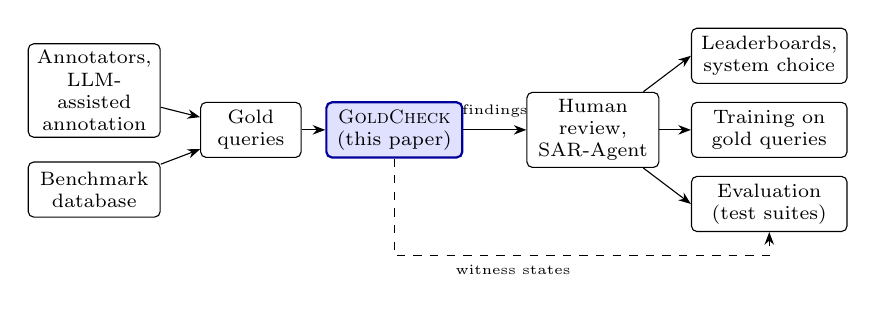
\begin{tikzpicture}[font=\scriptsize, node distance=3mm and 3mm,
  box/.style={draw, rounded corners=2pt, align=center, inner sep=2.5pt, minimum height=7mm},
  us/.style={box, fill=blue!12, draw=blue!60!black, thick},
  arr/.style={-{Stealth[length=1.6mm]}, thin}]
\node[box, text width=15mm] (ann) {Annotators,\\LLM-assisted\\annotation};
\node[box, text width=15mm, below=of ann] (db) {Benchmark\\database};
\node[box, text width=11mm, right=5mm of ann, yshift=-5mm] (gold) {Gold\\queries};
\node[us, text width=15.5mm, right=of gold] (gc) {\sys{}\\(this paper)};
\node[box, text width=15mm, right=8mm of gc] (rev) {Human review,\\SAR-Agent};
\node[box, text width=18mm, above right=1mm and 4mm of rev] (lb) {Leaderboards,\\system choice};
\node[box, text width=18mm, right=4mm of rev] (tr) {Training on\\gold queries};
\node[box, text width=18mm, below right=1mm and 4mm of rev] (ev) {Evaluation\\(test suites)};
\draw[arr] (ann) -- (gold); \draw[arr] (db) -- (gold);
\draw[arr] (gold) -- (gc); \draw[arr] (gc) -- node[above, font=\tiny, yshift=1pt]{findings} (rev);
\draw[arr] (rev) -- (lb.west); \draw[arr] (rev) -- (tr); \draw[arr] (rev) -- (ev.west);
\draw[arr, dashed] (gc.south) |- node[below, pos=0.7, font=\tiny]{witness states} ([yshift=-3mm]ev.south west) -- ([yshift=-3mm]ev.south) -- (ev.south);
\end{tikzpicture}}
\caption{Life cycle of a gold query and the position of \sys{}. The dashed
arrow marks witness states that can extend the evaluation.}
\label{fig:pipeline}
\end{figure}

\textbf{Upstream.} In Spider~\cite{yu2018spider} and BIRD~\cite{li2024bird},
annotators wrote a query and checked it on the benchmark database. Spider~2.0
moved to enterprise workflows~\cite{lei2025spider2}. Jin et al.\ propose SAPAR,
an annotation pipeline in which an LLM agent reviews each annotation and people
confirm or reject its diagnosis~\cite{jin2026pervasive}. In all of these, the
checks run on the database state that ships with the benchmark.

\textbf{Midstream.} Wretblad et al.\ found noisy questions and gold queries in
BIRD's financial database~\cite{wretblad2024noise}. Arcwise practitioners
re-checked Mini-Dev by hand~\cite{arcwise2024}. Jin et al.\ audited Mini-Dev and
Spider~2.0-Snow with SAR-Agent~\cite{jin2026pervasive}. In each step, SAR-Agent
proposes a verification query, runs it, and reads the result. At the end it
writes a report on correctness and ambiguity. With o3, SAR-Agent reached 83\%
precision on Mini-Dev at \$0.44 per example. GBV-SQL reports a typology of gold
errors that come from the SQL, the question, or the database~\cite{chen2026gbv}.
In machine learning, label errors in test sets are a known
problem~\cite{northcutt2021pervasive}. These methods are broad. They can find a
misread question or a wrong table. Their judgments come from people or from an
LLM, so they are costly, can vary from run to run, and need verification. \sys{}
is narrow and runs before them. It covers only state-dependent errors, but each
finding is reproducible and carries its own proof.

\textbf{Downstream.} Leaderboards rank systems by execution accuracy, and
experimental studies in the database community compare systems on
them~\cite{kim2020nl2sql,katsogiannis2023survey,li2024dawn,li2024codes}. Zhong
et al.\ showed that one database lets wrong predictions pass and built distilled
test suites of databases~\cite{zhong2020test}. Pourreza and Rafiei analyzed
acceptable predictions that the benchmark judged wrong~\cite{pourreza2023evaluating},
and FLEX uses an LLM to emulate expert judgment of
predictions~\cite{kim2025flex}. These works assume that the gold query is right
and improve how a scorer compares predictions with it. Gold queries also serve as
training data for fine-tuned systems such as CodeS~\cite{li2024codes}. A
state-dependent gold query misleads all of them. \sys{}'s latent witnesses are
test-suite states aimed at the gold, and a benchmark can add them to its
evaluation.

\textbf{Principles we borrow.} SQL equivalence is undecidable in general.
Cosette~\cite{chu2017cosette} and EQUITAS~\cite{zhou2019equitas} prove
equivalence for restricted fragments. XData generates databases that separate a
query from its likely mutants~\cite{chandra2015xdata}, and engine-testing tools
vary queries and states to find engine bugs~\cite{rigger2020pqs,rigger2020tlp}.
Data-cleaning research has shown that no single detector finds most errors and
that a review budget is best spent on a combination of
detectors~\cite{abedjan2016detecting,chu2016cleaning,rekatsinas2017holoclean,krishnan2016activeclean}.
\sys{} applies these ideas to a new target. It holds the engine fixed and asks
whether the benchmark data determine the result of the reference query.
Table~\ref{tab:approaches} summarizes the differences.

\begin{table}[t]
\caption{Approaches to checking gold queries. The cost of SAR-Agent with o3 is
the figure reported by its authors~\cite{jin2026pervasive}.}
\label{tab:approaches}
\centering
\footnotesize
\setlength{\tabcolsep}{3pt}
\begin{tabular}{@{}lccccc@{}}
\toprule
 & Scope & LLM & Determ. & Evidence & Cost/query \\
\midrule
Human review & broad & no & no & note & manual \\
SAR-Agent (o3) & broad & yes & no & report & \$0.44 \\
SAR-Agent (open) & broad & yes & no & report & 6--82\,s GPU \\
Static rules & narrow & no & yes & none & $<$1\,ms \\
Run once & narrow & no & yes & result & ms \\
Random states & narrow & no & seeded & witness & varies \\
\sys{} & narrow & no & yes & witness & 17\,ms \\
\bottomrule
\end{tabular}
\end{table}

\section{Solution Overview}
\label{sec:overview}

\sys{} takes a gold query $G$ and the path of its database $D$, and returns a
list of findings with evidence. Fig.~\ref{fig:overview} shows its five
components. (1) The \emph{parser} turns $G$ into a parse tree and checks that
printing the tree back gives the same result as $G$. (2) The \emph{reading
builder} rewrites the tree into the other reading $G_c$ of each supported
construct. It builds a tie-complete query for a top-$k$ cut and a
\texttt{COUNT(DISTINCT)} query for a count of a primary key over a join. (3)
The \emph{executor} runs $G$ and each $G_c$ on $D$ through a read-only
connection and compares the result sets. A difference is a live finding. (4)
The \emph{witness search} runs only when a top-$k$ query shows no difference on
$D$. It edits one cell in a temporary copy of one table and asks the executor to
run $G$ and $G_c$ again. A difference is a latent finding. (5) The
\emph{reporter} attaches to each finding the SQL of both readings and their
results, so that a reviewer can re-run the proof.

The components share one rule. \sys{} reports a finding only when the executor
has observed a difference on a concrete database state. A person then decides
whether the finding is an error.

\begin{figure}[t]
\centering
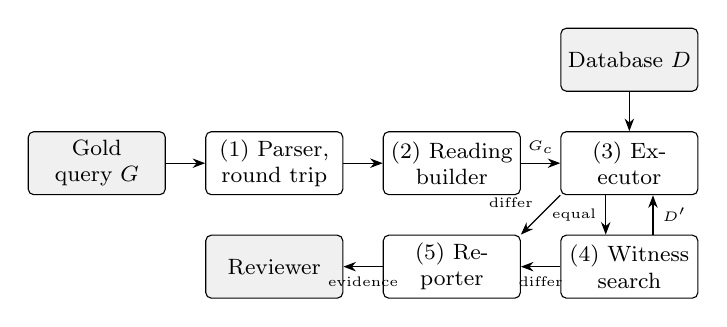
\begin{tikzpicture}[font=\footnotesize, node distance=5mm and 5mm,
  box/.style={draw, rounded corners=2pt, align=center, inner sep=2pt, minimum height=8mm, text width=16mm},
  io/.style={box, fill=black!6},
  arr/.style={-{Stealth[length=1.6mm]}, thin}]
\node[io] (g) {Gold query $G$};
\node[box, right=of g] (p) {(1) Parser,\\round trip};
\node[box, right=of p] (b) {(2) Reading\\builder};
\node[box, right=of b] (e) {(3) Executor};
\node[io, above=of e] (d) {Database $D$};
\node[box, below=of e] (w) {(4) Witness\\search};
\node[box, below=of b] (r) {(5) Reporter};
\node[io, below=of p] (h) {Reviewer};
\draw[arr] (g) -- (p); \draw[arr] (p) -- (b);
\draw[arr] (b) -- node[above, font=\tiny]{$G_c$} (e);
\draw[arr] (d) -- (e);
\draw[arr] ([xshift=-3mm]e.south) -- node[left, font=\tiny]{equal} ([xshift=-3mm]w.north);
\draw[arr] ([xshift=3mm]w.north) -- node[right, font=\tiny]{$D'$} ([xshift=3mm]e.south);
\draw[arr] (e.south west) -- node[above left=-1pt, font=\tiny]{differ} (r.north east);
\draw[arr] (w) -- node[below, font=\tiny]{differ} (r);
\draw[arr] (r) -- node[below, font=\tiny]{evidence} (h);
\end{tikzpicture}
\caption{Components of \sys{}. Grey boxes are the inputs and the consumer.
$G_c$ is the other reading of $G$, and $D'$ is $D$ with one cell edited.
``Equal'' and ``differ'' refer to the results of $G$ and $G_c$.}
\label{fig:overview}
\end{figure}

\section{The \sys{} Checker}
\label{sec:method}

\sys{} takes a gold query and the path of its SQLite database. It parses the
query with sqlglot~\cite{sqlglot}, runs it, and applies the checks below. It reports a finding
only with evidence obtained by running SQL. \sys{} makes every edit in
\texttt{TEMP} shadow tables on a read-only connection and rolls it back at the
end of a savepoint.

\textbf{Round trip.} Each check rewrites the parse tree and prints it as SQL. A
difference must come from the rewrite and not from the parser. \sys{} therefore
first prints the unmodified tree and runs it. If its result differs from the
original, \sys{} skips the structural checks. This happens for 3.3\% of the 2025
Dev gold queries.

\textbf{Top-$k$ cut.} If the outermost \texttt{SELECT} has
\texttt{ORDER BY $o$ LIMIT $k$}, \sys{} builds the tie-complete reading
\begin{lstlisting}
SELECT c1..cm FROM (SELECT <outputs> AS c1..cm,
  RANK() OVER (ORDER BY o) AS r FROM ... ) WHERE r <= k
\end{lstlisting}
which keeps every row tied with the $k$-th row, with the same filters, joins, and
grouping. \sys{} replaces sort keys that refer to output aliases by their
expressions. If $G_c(D) \supsetneq G(D)$, the gold drops tied rows whose output
differs, and \sys{} reports a \emph{top-$k$ tie} with the dropped rows. It also
re-runs the query without the limit and with the sort keys added to the output.
If the first key is \texttt{NULL}, it reports \emph{NULL at top}. \sys{} does
not rewrite queries with \texttt{DISTINCT} or \texttt{SELECT *} at the top
level.

\textbf{Count fan-out.} For every \texttt{COUNT($t.a$)} without
\texttt{DISTINCT} in a \texttt{SELECT} with joins, \sys{} checks whether $a$ is
the single-column primary key of $t$. If so, the author meant to count entities
of $t$, and a join can repeat them. \sys{} runs the query with
\texttt{COUNT(DISTINCT $t.a$)}. If the result changes, it reports a \emph{count
fan-out} with both values.

\textbf{Empty answer.} \sys{} reports an \emph{empty answer} if the gold
result has no rows or only \texttt{NULL} values.

\textbf{Targeted latent witnesses.} If the tie-complete reading returns the same
result as the gold, the official data have no harmful tie at the cut. \sys{}
then builds one with a single-cell edit. It requires every sort key to be a
plain column of one base table $T$. It runs the query without the limit and adds
the sort keys and the \texttt{rowid} of $T$ to the output. The first rows below
the cut are exactly the rows that a tie could promote. For each of up to six such
rows, \sys{} sets the sort key in a shadow copy of $T$ to the value of the $k$-th
row and runs $G$ and $G_c$. It stops at the first state on which they differ.
The witness records the table, the \texttt{rowid}, the column, the old and new
value, and both results. Consider \emph{``What is the phone number of the school
with the highest number of test takers scoring over 1500?''} Setting one
school's count from 2,125 to 5,837 makes the gold return one phone number and
the tie-complete reading two.

Algorithm~\ref{alg:goldcheck} summarizes the procedure, and
Fig.~\ref{fig:witness} shows a latent witness.

\begin{algorithm}[t]
\caption{\sys{} for one gold query}
\label{alg:goldcheck}
\footnotesize
\begin{algorithmic}[1]
\Require gold query $G$, official database $D$ (opened read-only)
\State $F \gets \emptyset$;\; $T \gets \textsc{Parse}(G)$;\; $R \gets G(D)$
\If{$R$ is empty or contains only \texttt{NULL}}
  \State $F \gets F \cup \{\textit{empty answer}\}$
\EndIf
\If{$\textsc{Print}(T)(D) \neq R$} \Return $F$ \Comment{round trip fails}
\EndIf
\If{$T$ has an outer \texttt{ORDER BY} $o$ \texttt{LIMIT} $k$}
  \State $G_c \gets \textsc{TieComplete}(T)$
  \If{$G_c(D) \supsetneq R$}
    \State $F \gets F \cup \{\textit{tie}: G_c(D) \setminus R\}$
  \EndIf
  \If{the first sort key without the limit is \texttt{NULL}}
    \State $F \gets F \cup \{\textit{NULL at top}\}$
  \EndIf
  \If{$G_c(D) = R$ and $o$ are plain columns of a base table $B$}
    \State copy $B$ into a \texttt{TEMP} shadow table, keeping \texttt{rowid}
    \For{each of the first six rows $r$ below the cut}
      \State savepoint; set $r.o$ to the sort key of the $k$-th row
      \If{$G(D') \neq G_c(D')$}
        \State $F \gets F \cup \{\textit{latent}: (B, r, o)\}$; \textbf{break}
      \EndIf
      \State rollback
    \EndFor
  \EndIf
\EndIf
\For{each \texttt{COUNT($t.a$)} without \texttt{DISTINCT} under a join}
  \If{$a$ is the one-column primary key of $t$}
    \If{$G$ with \texttt{COUNT(DISTINCT $t.a$)} returns $\neq R$}
      \State $F \gets F \cup \{\textit{fan-out}\}$
    \EndIf
  \EndIf
\EndFor
\State \Return $F$, each finding with the SQL and results that prove it
\end{algorithmic}
\end{algorithm}

\begin{figure}[t]
\centering
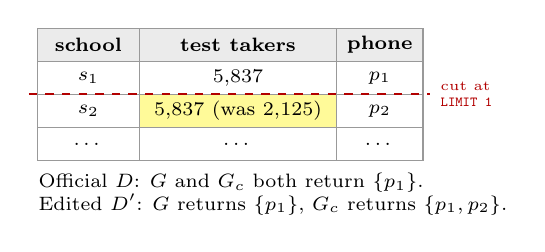
\begin{tikzpicture}[font=\scriptsize,
  cell/.style={draw=black!40, minimum height=4.2mm, inner sep=1.5pt, anchor=west},
  hd/.style={cell, fill=black!8, font=\scriptsize\bfseries}]
\node[hd, minimum width=13mm] at (0,0) {school};
\node[hd, minimum width=25mm] at (13mm,0) {test takers};
\node[hd, minimum width=11mm] at (38mm,0) {phone};
\node[cell, minimum width=13mm] at (0,-4.2mm) {$s_1$};
\node[cell, minimum width=25mm] at (13mm,-4.2mm) {5,837};
\node[cell, minimum width=11mm] at (38mm,-4.2mm) {$p_1$};
\node[cell, minimum width=13mm] at (0,-8.4mm) {$s_2$};
\node[cell, minimum width=25mm, fill=yellow!40] at (13mm,-8.4mm) {5,837 (was 2,125)};
\node[cell, minimum width=11mm] at (38mm,-8.4mm) {$p_2$};
\node[cell, minimum width=13mm] at (0,-12.6mm) {\ldots};
\node[cell, minimum width=25mm] at (13mm,-12.6mm) {\ldots};
\node[cell, minimum width=11mm] at (38mm,-12.6mm) {\ldots};
\draw[red!70!black, thick, dashed] (-1mm,-6.3mm) -- (50mm,-6.3mm)
  node[right, font=\tiny, text=red!70!black, align=left] {cut at\\\texttt{LIMIT 1}};
\node[anchor=north west, align=left] at (-1mm,-15.1mm)
  {Official $D$: $G$ and $G_c$ both return $\{p_1\}$.\\
   Edited $D'$: $G$ returns $\{p_1\}$, $G_c$ returns $\{p_1, p_2\}$.};
\end{tikzpicture}
\caption{A latent witness for the phone number of the school with the most test
takers over 1500, with schools and phone numbers abbreviated.}
\label{fig:witness}
\end{figure}

\textbf{Design choices.} Three choices keep findings few and meaningful. First,
a tie counts only if the tied rows differ in the output columns. Ties at the cut
are common, and many are harmless. Two rows of the same entity can share a sort
key and print the same answer. Second, a fan-out counts only
when the counted column is the primary key of its table. Counting a primary key
signals that the author meant to count entities, so a join that repeats them
changes the meaning. Counting a non-key column over a join is often deliberate.
Third, \sys{} edits only rows just below the cut, and only their sort key. Only
such edits can change which rows survive the cut, so only they can create a tie
there. Our experiments measure the first and third choices.

\textbf{Complexity.} Let $T_G$ be the time to run $G$ on $D$. \sys{} runs $G$
once, its printed tree once, the tie-complete reading once, the unlimited probe
once, and one \texttt{DISTINCT} reading per counted primary key. The witness
search adds at most six edits with two runs each and one copy of the base table
$B$. The total is at most $(16 + c)$ query executions, where $c$ is the number
of counted primary keys, plus $O(|B|)$ for the copy. The cost is therefore
linear in the cost of the gold query itself and does not depend on the number of
gold queries checked before.

\textbf{Guarantees and limits.} \sys{} observes every reported difference on a
concrete database state, so its findings are sound by construction. \sys{} does
not judge which reading the question intends and does not prove equivalence. It
misses differences that its rewrites and edits do not reach. It does not look
for errors that are unrelated to the data, such as a wrong table or a misread
question. \sys{} is about 240 lines of Python on top of sqlglot and the
\texttt{sqlite3} module. It registers an \texttt{IIF} function, which our SQLite
version 3.31 lacks.

\section{Experimental Evaluation}
\label{sec:eval}

\subsection{Releases}
Table~\ref{tab:corpus} lists the releases we align. For Mini-Dev, three
versions of the same 498 SQLite examples exist. T0 is the gold shipped by BIRD.
T1 is a community correction by practitioners at Arcwise~\cite{arcwise2024}. T2
is the research audit of Jin et al.~\cite{jin2026pervasive}. The audit started
from T1 and released a per-example diff. We verified that its recorded starting
point equals T1 for all 498 examples. For the full Dev set, two versions exist.
They are the 2024-06-27 gold and the maintainers' review of
2025-11-06~\cite{bird2025dev}. BIRD drew Mini-Dev from Dev. We call the other
1,036 Dev examples \emph{held-out}, and we built no definition by looking at
them. A 2026 Mini-Dev release~\cite{bird2026minidev} rewrote and renumbered the
questions, so we cannot align it. We also use Dev-100. It consists of 100 Dev
questions that Jin et al.\ corrected, with predictions from 16 published
systems~\cite{jin2026pervasive}.

\begin{table}[t]
\caption{Aligned releases. ``Changed'' counts gold queries whose normalized text
differs. ``Output'' counts those whose two versions return different result
sets.}
\label{tab:corpus}
\centering
\footnotesize
\begin{tabular}{@{}lrrr@{}}
\toprule
Review, old to new & $n$ & Changed & Output \\
\midrule
Mini-Dev T0 to T1, community & 498 & 97 & 89 \\
Mini-Dev T1 to T2, research audit & 498 & 134 & 75 \\
Dev 2024 to 2025, maintainers & 1,534 & 396 & 252 \\
\quad held-out, not in Mini-Dev & 1,036 & 273 & 176 \\
Dev-100 old to corrected, audit & 100 & 69 & 19 \\
\bottomrule
\end{tabular}
\end{table}

A changed gold query is not always a wrong one. Reviewers also rename output
columns and rewrite for style. We therefore use the stricter outcome, a change of
output, wherever it matters. To compare text, we parse both versions with
sqlglot in the SQLite dialect and print them in canonical form.

\subsection{Methods and measures}
\textbf{Releases and references.} We run every method on the version under
review in each of three human reviews (Table~\ref{tab:corpus}). We then count how
often the review changed the output of the queries the method flags. None of the
reviews used any of the methods. The maintainers' Dev review is the cleanest
reference. Mechanisms we saw in the Mini-Dev audit motivated our classes, and Dev contains 1,036 examples outside Mini-Dev that we did not inspect when we chose the classes. We report results on these held-out examples separately as an out-of-sample test.

\textbf{Methods.} We chose baselines by one criterion. Each removes one
ingredient of \sys{} or represents a published way to check or test queries.
The first three are our own constructions and do not stand for a published
system. (1) \emph{Static rules} read the SQL without running it. They
flag the same constructs as \sys{}, a top-level \texttt{ORDER BY \ldots{} LIMIT}
and a \texttt{COUNT} of a column without \texttt{DISTINCT} over a join. (2)
\emph{Run once} mirrors what an annotator sees. It flags a gold query that fails,
returns nothing, returns duplicate rows, or returns a \texttt{NULL}. (3)
\emph{Random edits} replace \sys{}'s targeted witness search with random edits in
the style of test suites. Each try sets the sort key of a random row to the
boundary value. (4) \emph{SAR-Agent}~\cite{jin2026pervasive} runs with its released prompt and loop on open models. This re-run is not the published system, which uses o3, and we label it as an open-model re-run throughout.

\textbf{Measures.} For a set of flagged queries, we report the share whose
output the next review changed. We divide this share by the share among all
other queries and call the ratio \emph{lift}. We also report the recall of all
output changes, and we report cost as time per query. Lift is a ratio, so we checked its denominator. The share among unflagged queries lies between 14\% and 16\% in the three reviews and is never close to zero. We report the absolute shares next to each lift and give 95\% intervals from 2,000 bootstrap resamples of the queries~\cite{efron1979bootstrap}. Figures show Wilson intervals~\cite{wilson1927}.

\subsection{Agreement with human reviews}
Table~\ref{tab:baselines} gives the results. \sys{} flags few queries, and the
reviews changed many of them. They changed the output of 56\%, 57\%, and 35\% of
flagged queries, against 14\% to 15\% of the rest. The lift is 3.7, 4.1, and
2.3. Static rules flag 4.7 to 11 times as many queries, with a lift of 1.4, 1.0,
and 1.6. A top-$k$ cut or a count over a join is common and usually harmless.
What matters is whether the data make the reading matter, and only execution
shows that. Running the gold once gives a lift of 1.0 to 1.7. Fig.~\ref{fig:agreement}
shows the \sys{} rates with intervals.

\textbf{Uncertainty and out-of-sample test.} The 95\% bootstrap intervals of
the \sys{} lift are 2.5 to 5.3, 2.1 to 6.5, and 1.7 to 3.0 for the three
reviews. The intervals of run once are 0.5 to 2.0, 0.8 to 2.8, and 0.7 to 1.5,
and those of static rules are 1.0 to 2.1, 0.6 to 1.5, and 1.2 to 2.0. On the
1,036 held-out Dev examples, \sys{} flags 72 queries. The review changed the
output of 27 of them (37.5\%) and of 149 of the other 964 (15.5\%). The lift is
2.4, with an interval from 1.7 to 3.3. Static rules reach 1.7 there (1.3 to 2.3)
and run once 1.0 (0.6 to 1.5). The intervals of \sys{} and static rules overlap
on the maintainers' review, so on that review we can only state that \sys{}
flags one fifth as many queries at a higher changed share (35.2\% against
21.9\%).

\begin{table}[t]
\caption{Gold queries flagged per method. Out\% is the share whose output the
next review changed, lift is its ratio to unflagged queries, and recall covers
all output changes. Bold marks the highest value per review.}
\label{tab:baselines}
\centering
\footnotesize
\setlength{\tabcolsep}{3.2pt}
\begin{tabular}{@{}llrrrr@{}}
\toprule
Review & Method & Flagged & Out\% & Lift & Recall \\
\midrule
Community & Static rules & 175 & 22.3 & 1.44 & 39/89 \\
(Mini-Dev T0) & Run once & 40 & 20.0 & 1.13 & 8/89 \\
 & \sys{} & 32 & \textbf{56.2} & \textbf{3.69} & 18/89 \\
\midrule
Research audit & Static rules & 154 & 14.9 & 0.99 & 23/75 \\
(Mini-Dev T1) & Run once & 38 & 23.7 & 1.65 & 9/75 \\
 & \sys{} & 14 & \textbf{57.1} & \textbf{4.13} & 8/75 \\
\midrule
Maintainers & Static rules & 498 & 21.9 & 1.59 & 109/252 \\
(Dev 2024) & Run once & 157 & 17.2 & 1.05 & 27/252 \\
 & \sys{} & 105 & \textbf{35.2} & \textbf{2.34} & 37/252 \\
\bottomrule
\end{tabular}
\end{table}

\begin{figure}[t]
\centering
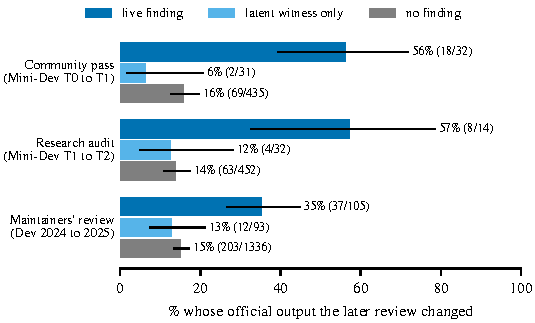
\includegraphics[width=\columnwidth]{figures/fig_agreement.pdf}
\caption{Share of gold queries whose output the next human review changed, by
\sys{} result on the version under review, with 95\% Wilson intervals.}
\label{fig:agreement}
\end{figure}

Latent witnesses behave differently. The reviews changed queries whose only
finding is latent at or below the base rate, at 6\%, 12\%, and 13\%. Reviewers do
not treat a top-$k$ query as wrong when the data happen to have no tie. This
matches the definition. A latent finding shows that the test is weak, not that
the gold is wrong.

\subsection{Survival of findings across reviews}
\label{sec:survival}
Fig.~\ref{fig:fate} follows each live finding into the next version, and
Table~\ref{tab:findings} counts findings per release. The two Mini-Dev reviews
together removed 29 of 34 findings, including 12 of 13 ties and 14 of 17 count
fan-outs. The maintainers' Dev review removed 47 of 110 and none of the eight
empty answers. Of the 65 Dev queries with a live finding in the 2025 release,
\sys{} had already flagged 60 in 2024. The review left 55 of them word for word
unchanged. Five findings remain in Mini-Dev after the audit that SAR-Agent
assisted. Two are clear errors. In one, the gold picks the first race of the
youngest driver from tied rows rather than by date. The other three are counts
meant to count join rows.

\begin{figure}[t]
\centering
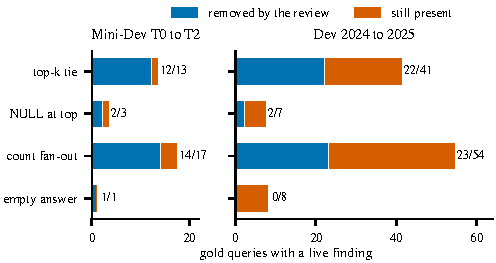
\includegraphics[width=\columnwidth]{figures/fig_fate.pdf}
\caption{Live findings per class in the version under review, split by whether
the next version still has them.}
\label{fig:fate}
\end{figure}

\begin{table}[t]
\caption{\sys{} findings per release. A query can have several findings.}
\label{tab:findings}
\centering
\footnotesize
\setlength{\tabcolsep}{4pt}
\begin{tabular}{@{}lrrrrr@{}}
\toprule
 & \multicolumn{3}{c}{Mini-Dev (498)} & \multicolumn{2}{c}{Dev (1,534)} \\
\cmidrule(lr){2-4}\cmidrule(l){5-6}
Finding & T0 & T1 & T2 & 2024 & 2025 \\
\midrule
Top-$k$ tie & 13 & 8 & 1 & 41 & 21 \\
\texttt{NULL} at top & 3 & 1 & 1 & 7 & 5 \\
Count fan-out & 17 & 5 & 3 & 54 & 32 \\
Empty answer & 1 & 0 & 0 & 8 & 10 \\
\midrule
Queries with a live finding & 32 & 14 & 5 & 105 & 65 \\
Queries with a latent witness & 31 & 32 & 29 & 93 & 77 \\
\midrule
Top-$k$ queries & 75 & 74 & 68 & 250 & 240 \\
Skipped (parser round trip) & 26 & 25 & 23 & 56 & 51 \\
\bottomrule
\end{tabular}
\end{table}

The 65 findings in the latest release are what \sys{} would hand to the next
reviewer. For 31 of them, 21 ties and 10 empty answers, the test is defective
whatever the question intends. A tie leaves the answer to the engine, and an empty answer accepts any query that matches
nothing. For the 32 fan-outs and the 5 \texttt{NULL} tops, the intent decides.
Two authors judged these 37 findings independently from the question and its
evidence note, without seeing each other's labels. They agreed on 33 of the 37,
with a Cohen's $\kappa$~\cite{cohen1960kappa} of 0.60 and a 95\% bootstrap interval from 0.16 to 0.92. The interval is wide because only 37 items were judged. The $\kappa$ is lower than the raw agreement
because most findings are errors, which raises chance agreement. Both judged all
5 \texttt{NULL} tops to be errors. Of the 32 fan-outs, both judged 24 to be
errors and 4 to be acceptable. They disagreed on 4, and three of these are
ratios whose other reading exceeds 100\%. We leave these 4 unresolved.
In total, 57 of the 65 flagged queries are a defective test or an error on which both annotators agree. Typical acceptable cases are counts
meant to count join rows. In \emph{``How many posts did Jay Stevens have in 2010?''}, counting a
user identifier over the posts table yields the number of posts.

\subsection{Findings in the latest release}
\label{sec:latest}
Table~\ref{tab:cases} shows typical findings in the 2025 release. By database,
the share of questions with a finding ranges from 1.6\% for the superhero
database to 11.0\% for the thrombosis database. Three patterns stand out.

\begin{table*}[t]
\caption{Typical \sys{} findings in the 2025-11-06 BIRD Dev release, with
abridged questions and the results of the gold query and of its other reading. A dash means that the class has no other reading.}
\label{tab:cases}
\centering
\footnotesize
\setlength{\tabcolsep}{4pt}
\newcolumntype{L}[1]{>{\raggedright\arraybackslash}p{#1}}
\begin{tabular}{@{}rL{5.6cm}lL{2.3cm}L{1.9cm}L{3.6cm}@{}}
\toprule
ID & Question & Class & Gold & Other reading & Comment \\
\midrule
802 & Who is the tallest superhero? & tie & Surtur & Surtur, Ymir & two heroes share the height \\
\rowsep
766 & Full name of the hero with the highest strength & tie & 1 name & 36 names & 36 heroes share the top value \\
\rowsep
1002 & Youngest racer and the race she first joined & tie & 1 race & 13 races & ordered by birth date only, not by race date \\
\rowsep
1196 & Most common sign of patients with SLE & tie & 1 sign & 4 signs & four signs share the top count \\
\rowsep
37 & Address of the school with the lowest excellence rate & \texttt{NULL} top & a school with no rate & 561 such schools & the ``lowest'' rate is missing \\
\rowsep
1203 & Female patients with white blood cells below 3.5 & fan-out & 641 & 88 & counts lab tests, not patients \\
\rowsep
1308 & Patients with a normal platelet level and other symptoms & fan-out & 10,079 & 294 & counts lab tests, not patients \\
\rowsep
150 & Accounts in North Bohemia with a transaction to bank AB & fan-out & 2,260 & 55 & counts transactions, not accounts \\
\rowsep
677 & How many posts did Jay Stevens have in 2010? & fan-out & 3 & 1 & acceptable, posts are meant \\
\rowsep
936 & Fastest lap of Lewis Hamilton in the 2008 Australian GP & empty & no rows & -- & any prediction with no rows scores \\
\rowsep
1504 & Average total price of transactions in January 2012 & empty & \texttt{NULL} & -- & any average over no rows scores \\
\bottomrule
\end{tabular}
\end{table*}

First, one database dominates. The thrombosis database holds 18 of the 65
findings. Its patients have many lab tests each, and most of its findings are
fan-outs over the join of patients and lab tests. Its questions ask about patients, but its gold queries
often count lab rows. The database had 24 fan-outs in 2024 and still has 14.

Second, ties at the top are not rare corner cases. In 10 of the 21 tie findings,
the gold keeps one row while two to four rows share the top value. In eight more,
the tied group is larger, up to 561 rows. In the remaining three, the cut is at
$k=5$ or $k=10$. A system that answers the question as asked lists all tied rows,
and it receives no credit in any of these cases.

Third, empty answers cluster. Six of the ten ask about the 2008 or 2011
Australian Grand Prix in the motorsport database. Empty answers grew from eight
to ten in the review, and the review changed the output of none of the eight.
Editing the query cannot repair an empty answer. The question or the data must
change.


Findings are not concentrated in hard questions. By BIRD's difficulty label,
3.6\% of simple, 6.3\% of moderate, and 2.6\% of challenging questions have a live
finding. A tie or a fan-out is as easy to write in a one-line query as in a
nested one.

\subsection{Targeted versus random state edits}
Test suites search for distinguishing states by sampling~\cite{zhong2020test}.
\sys{} attempted a witness on 116 Dev 2025 top-$k$ queries. Its targeted search
edits only rows just below the cut, and it found a witness for 77 with at most
six one-cell edits. Random one-cell edits found 35 with one try, 52 within ten,
and 66 within 100. They found nine witnesses that the targeted search missed and
missed 20 that it found. A likely reason is that the edit that matters is predictable. It must promote a row that differs in output to the boundary, and a random row is often one that the query filters out. We did not test this explanation separately.

\subsection{Contribution of each design choice}
\label{sec:ablation}
Table~\ref{tab:perclass} breaks the agreement down by class. Ties and fan-outs
carry most of the signal in every review. The research audit changed six of the
eight ties that the community review had left. The maintainers changed the output of 14
of 41 ties and 23 of 54 fan-outs, against 15\% of queries without a finding.

\begin{table}[t]
\caption{Changed in output by the next review, of the queries flagged per class.
Entries are changed/flagged, and a dash means not measured. $^{*}$Ties whose rows print the same answer, which \sys{} does not flag.}
\label{tab:perclass}
\centering
\footnotesize
\setlength{\tabcolsep}{3.5pt}
\begin{tabular}{@{}lrrr@{}}
\toprule
Class & Community & Audit & Maintainers \\
 & (T0) & (T1) & (Dev 2024) \\
\midrule
Top-$k$ tie & 5/13 & 6/8 & 14/41 \\
\texttt{NULL} at top & 2/3 & 0/1 & 2/7 \\
Count fan-out & 12/17 & 2/5 & 23/54 \\
Empty answer & 1/1 & -- & 0/8 \\
\midrule
Latent witness & 2/31 & 4/32 & 12/93 \\
Tie, same output$^{*}$ & -- & -- & 1/20 \\
\bottomrule
\end{tabular}
\end{table}

\textbf{Requiring a difference in output.} In Dev 2024, 20 gold queries cut at a
tie whose rows all print the same answer. An example is two lab records of the
same patient with the same value. \sys{} does not flag them. The review changed
the output of one of them (5\%), against 14 of 41 (34\%) for ties whose rows
differ. Flagging
every tie would add 20 queries and lower the share of changed queries among tie
flags from 34\% to 25\%.

\textbf{Requiring execution.} Static rules flag the same constructs without
running them (Table~\ref{tab:baselines}). They flag 4.7 to 11 times as many
queries, and their lift falls to between 1.0 and 1.6. The construct alone is
weak evidence. The data decide whether it matters.

\subsection{Engine dependence of tie answers}
\label{sec:engines}
Section~\ref{sec:engine} argued that a tie at the cut leaves the gold answer to
the engine. We tested this directly. We ran every gold query with a live tie,
unchanged, under four conditions that keep the data identical
(Table~\ref{tab:engines}). The first reverses the scan order of SQLite with
\texttt{PRAGMA reverse\_unordered\_selects}. The second rebuilds every table the
query reads in reverse row order, without indexes. The third rebuilds the tables
in the original row order, which isolates the effect of the indexes. The fourth
runs DuckDB~1.1.3~\cite{raasveldt2019duckdb} on the same SQLite file.

\begin{table}[t]
\caption{Gold queries whose result changed on identical data. DuckDB failed on
4 of 21 and 8 of 41 tie queries and is omitted for controls (dash). Numbers in parentheses are group sizes.}
\label{tab:engines}
\centering
\footnotesize
\setlength{\tabcolsep}{3pt}
\begin{tabular}{@{}lrrrr@{}}
\toprule
 & Reverse & Rebuilt, & Rebuilt, & DuckDB \\
 & scan & reverse & same order & \\
\midrule
Tie, Dev 2025 (21) & 0 & 11 & 3 & 4 \\
Tie, Dev 2024 (41) & 0 & 23 & 6 & 7 \\
No tie at cut, 2025 (206) & 1 & 2 & 0 & -- \\
No tie at cut, 2024 (198) & 1 & 3 & 0 & -- \\
\bottomrule
\end{tabular}
\end{table}

In the 2025 release, rebuilding the tables in reverse order changed the gold
answer of 11 of the 21 tie queries, and every new answer is another tied row.
Dropping the indexes alone changed three. DuckDB returned another tied row for
four of the 17 tie queries it could run. Over the three SQLite conditions, 12 of
the 21 gold answers changed. In the 2024 release, 24 of 41 changed. Reversing the scan order changed none of them. Whether a tie flips thus depends on storage and plan details that the gold query does not control.

Among the 206 top-$k$ gold queries without a tie at the cut, the SQLite
conditions changed two. Both are state-dependent in another way. They select a
column that is neither grouped nor aggregated, and SQLite takes its value from
an arbitrary row. This construct is outside the four classes of \sys{}.

\subsection{LLM reviewers of growing size}
\label{sec:llm}
If state-dependent gold queries were only a matter of reviewer skill, a larger
model would remove them. We test this with SAR-Agent. Its released code calls
OpenAI o3. To avoid API cost, we re-ran its released prompt and loop with open
models from 3B to 120B parameters, Qwen2.5~\cite{qwen2024qwen25,hui2024qwen25coder} and gpt-oss~\cite{openai2025gptoss}, served by vLLM~\cite{kwon2023vllm} and Ollama~\cite{ollama}. The result describes these open models and does not transfer to o3, which we did not run. Three changes were
unavoidable. The authors did not release the per-database schema file, so we
rebuild it from the \texttt{CREATE} statements and BIRD's column descriptions.
Not every open model supports OpenAI function calling, so every model emits each
call as one JSON object per reply. The released code opens the database writable
and executes model-written SQL, so we run queries on a read-only connection. We
review 300 Dev 2024 gold queries, the 105 with a live \sys{} finding and 195
random others. For each finding, we ask whether SAR-Agent judged the gold wrong
\emph{and} named the mechanism in its explanation.

\begin{table}[t]
\caption{SAR-Agent on the 105 Dev 2024 gold queries with a live finding.
``+ev.'' adds the \sys{} evidence. ``Named'' means judged wrong with the mechanism named, by keyword match. Numbers in parentheses are class sizes, and a dash means not run.}
\label{tab:sar}
\centering
\footnotesize
\setlength{\tabcolsep}{2.4pt}
\begin{tabular}{@{}lrrrrrr@{}}
\toprule
 & \multicolumn{3}{c}{Qwen2.5} & gpt-oss & 32B & 120B \\
\cmidrule(lr){2-4}\cmidrule(lr){5-5}\cmidrule(l){6-7}
Named, by class & 3B & 7B & 32B & 120B & +ev. & +ev. \\
\midrule
Count fan-out (54) & 6 & 3 & 19 & 43 & 49 & 46 \\
Top-$k$ tie (41) & 1 & 3 & 10 & 11 & 27 & 37 \\
Empty answer (8) & 3 & 6 & 4 & 3 & 5 & 5 \\
\texttt{NULL} at top (7) & 0 & 0 & 0 & 2 & 6 & 5 \\
\midrule
Judged wrong (of 105) & 39 & 28 & 59 & 79 & 100 & 95 \\
Mean steps & 3.9 & 3.3 & 4.1 & 1.3 & -- & -- \\
Same verdict (of 50) & 33 & -- & 36 & -- & -- & -- \\
Mean latency (s) & 17.0 & 6.0 & 81.5 & 18.7 & -- & -- \\
\bottomrule
\end{tabular}
\end{table}

\textbf{Fan-outs and ties respond differently to model size.}
Table~\ref{tab:sar} shows the result. As the model grows, SAR-Agent names more
fan-outs. It names 6 of 54 with the 3B model and 43 of 54 with the 120B model. A
reader can see a fan-out in the SQL text as a \texttt{COUNT} over a join without
\texttt{DISTINCT}. Ties do not follow. From
32B to 120B, the count of named ties barely moves, from 10 to 11 of 41. Neither
the query nor its result shows a tie. The reviewer sees one row and has to
suspect that the cut dropped a second row with the same value. Then the
reviewer has to write a query to check. The 120B model took 1.3 steps per review
on average, including the final verdict. It rarely ran a verification query and
judged mostly by reading. The smaller models ran queries but did not look for
ties. For \emph{``Who is the tallest superhero?''} the 3B model ran the
gold, saw one name, and wrote that ``the result [(`Surtur',)] confirms that
Surtur is the tallest superhero according to the given data.'' For the 641
patients it wrote that the count ``matches the expected count based on the
conditions provided.''

Latent findings are out of reach for a reviewer that only queries the official database. On the official
database, the gold and its other reading agree, so no query a reviewer runs there
can show a difference. The difference exists only on a database that the
reviewer never sees.

\textbf{Verdicts vary between runs.} On 50 queries reviewed twice with the same
model and settings, the verdicts agreed on 33 (Cohen's $\kappa=0.30$) with the 3B
model and on 36 ($\kappa=0.47$) with the 32B model. \sys{} gives the same output
on every run.

\textbf{\sys{} as input to a reviewer.} Because the two do different jobs, the
natural use is to run \sys{} first and hand its evidence to whoever judges the
question, a person or an LLM. We re-ran SAR-Agent on the 105 findings with the
\sys{} evidence appended to its prompt (Table~\ref{tab:sar}, right). The
evidence lists the tied rows that the gold cuts off, or the two counts, as
results of running SQL. A note says that the evidence does not tell which
reading the question intends. With the
evidence, the 32B model named the tie in 27 of 41 findings instead of 10, and
the 120B model in 37 instead of 11. The 32B model with evidence named 87 of the
110 mechanisms, more than the 120B model without it (59). In these runs, adding the evidence raised the number of named ties more than a fourfold increase in model size did.

The evidence does not settle the reading. With it, both models judged almost
every flagged gold query wrong, 100 and 95 of 105, whereas the maintainers
changed the output of about a third. The 120B model kept 10 gold queries as
correct, and the review changed none of them. Ten cases are too few to read much
into. Whether a finding is an error depends on what the question intends. For
this reason, \sys{} reports evidence and leaves the decision to a person.

\subsection{Case study: scores of model predictions}
\label{sec:downstream}
A finding matters downstream only if systems actually write the other reading.
We asked four open models of growing size to write one SQLite query for each of
the 1,534 questions of the 2025 release. The prompt is zero-shot and contains the
schema with BIRD's column descriptions and the evidence note, and the
temperature is 0. We scored the predictions in two ways
(Table~\ref{tab:downstream}). The first is BIRD's rule. The second also accepts
the other reading of a flagged gold query.

\begin{table}[t]
\caption{Predictions of four open models on the 2025 Dev release, scored by
BIRD's rule and by a rule that also accepts the other reading of the 65 flagged
gold queries.}
\label{tab:downstream}
\centering
\footnotesize
\setlength{\tabcolsep}{3pt}
\begin{tabular}{@{}lrrrr@{}}
\toprule
 & \multicolumn{3}{c}{Qwen2.5} & gpt-oss \\
\cmidrule(lr){2-4}\cmidrule(l){5-5}
 & 3B & 7B & 32B & 120B \\
\midrule
Accuracy, BIRD rule (\%) & 25.3 & 40.8 & 57.4 & 52.6 \\
Accuracy, either reading (\%) & 25.4 & 41.1 & 58.4 & 53.5 \\
\midrule
\multicolumn{5}{@{}l}{On the 65 flagged questions} \\
\quad scored correct, BIRD rule & 9 & 14 & 20 & 16 \\
\quad\quad of them empty answers & 3 & 7 & 9 & 9 \\
\quad wrote the other reading & 2 & 5 & 16 & 13 \\
\quad\quad \texttt{COUNT(DISTINCT)} (of 32) & 1 & 2 & 13 & 11 \\
\quad\quad another or every tied row (of 21) & 1 & 3 & 3 & 2 \\
\bottomrule
\end{tabular}
\end{table}

The two larger models wrote the other reading more often than the two smaller ones. On the 32 fan-out questions, the 32B model counted
distinct entities 13 times and counted join rows, as the gold does, 6 times. The
120B model did so 11 and 4 times. BIRD's rule rejects every one of those 24
entity counts. Across the 65 flagged questions, the number of predictions that
match the other reading grows from 2 for the 3B model to 16 and 13 for the two
strongest. For those two, it exceeds the number of flagged non-empty questions
they get right under BIRD's rule, 11 and 7. Empty answers work the other way.
Both strong models score 9 of the 10, although the database holds no answer to
any of them.

Over the whole release, the effect is about one point of accuracy, because the
findings cover 4\% of the questions. It does not reorder these four models. The
second rule is an upper bound. It also accepts the other reading where the gold
reading is the intended one, as for the posts of Jay Stevens. This case study covers four zero-shot models and no published system, so it shows that the other reading occurs in real predictions and does not establish a trend with model quality.

\subsection{Coverage and cost}
\label{sec:coverage}
\sys{} covers a narrow slice by design. Its live findings flag 11\% to 20\% of
the output changes made by each review (Table~\ref{tab:baselines}). This matches
the share of state-dependent mechanisms among the 134 research-audit corrections
that we coded (Table~\ref{tab:taxonomy}). Ties and missing \texttt{DISTINCT}
after a fan-out account for 19 of them (14\%). Most corrections fix a wrong
table, a wrong filter, or a misread domain rule, and no data-only check can find
these. \sys{} should therefore run before a broad review, not instead of it.

On the latest Dev release, \sys{} needs a median of 17\,ms per query. The 95th
percentile is 1.4\,s, and the slowest query takes 37\,s because the gold query
itself is slow. The release takes 637 CPU seconds, about one minute on ten
cores. \sys{} does not attempt a witness for 87 top-$k$ queries whose sort key is
an expression or a column of a common table expression.

\begin{table}[t]
\caption{The 134 research-audit corrections of Mini-Dev, coded by the audit's
four error classes~\cite{jin2026pervasive} and by mechanism, top eight of 42.
Bold mechanisms are in the scope of \sys{}.}
\label{tab:taxonomy}
\centering
\footnotesize
\begin{tabular}{@{}lr@{}}
\toprule
Error class & $n$ (\%) \\
\midrule
Misunderstanding of data or schema & 92 (69) \\
Domain-knowledge error & 23 (17) \\
Question and SQL logic do not match & 17 (13) \\
Output format & 2 (1) \\
\midrule
Mechanism & $n$ \\
\midrule
Age computed by year subtraction only & 15 \\
Missing filter for rows of the wrong kind or \texttt{NULL} & 14 \\
\textbf{Top-row selection ignores ties} & 10 \\
\textbf{Missing \texttt{DISTINCT} after a fan-out join} & 9 \\
Wrong source table & 9 \\
Aggregation at the wrong grain & 5 \\
Placeholder value treated as data (0 or `-') & 5 \\
Domain rule not applied & 5 \\
\bottomrule
\end{tabular}
\end{table}

\subsection{Case study: the training split}
\label{sec:train}
Gold queries also serve as training data for fine-tuned systems. We ran \sys{} unchanged on the BIRD training split.
The split has 9,428 gold queries over 69 databases, and we had looked at none of
them before. The run took 16 minutes on 12 cores, with a median of 11\,ms per
query.

Of the 9,428 gold queries, 780 (8.3\%) have a live finding. They comprise 337
empty answers, 260 ties at the cut, 183 count fan-outs, and 16 \texttt{NULL}
tops. Another 476 have a latent witness. Findings occur in 67 of the 69
databases. The rate is higher than in Dev before its review (6.8\%) and about
twice the rate in Dev after it (4.2\%). The training split has had no comparable
review. The run also exposed a problem of another kind. In total, 367 training
gold queries do not run at all, and 330 of them come from one database,
\texttt{retail\_world}. Its gold queries name tables and columns that its
database does not contain, in 330 of its 373 queries. We did not measure the effect of these pairs on a fine-tuned system.

\section{Execution Results of Corrected Gold Queries}
\label{sec:why}


We ran every old and new gold pair on the official database
(Fig.~\ref{fig:execution}). On Mini-Dev, either review later changed 201
original gold queries. Of these, 93.5\% run without error, return at least one
row, and return as many columns as their replacement. Under BIRD's own scoring
rule, 50 of the 201 (24.9\%) return the same result set as the corrected query.
On held-out Dev, 97 of 273 (35.5\%) do. In the research audit alone, 59 of its
134 SQL corrections leave the result set unchanged. Such corrections cannot
change any score under the benchmark's metric. Readers of error rates such as
52.8\% should keep this in mind, and that rate also counts ambiguous
questions~\cite{jin2026pervasive}. A reviewer who checks the old gold by running
it sees the same answer as after the fix.

\begin{figure}[t]
\centering
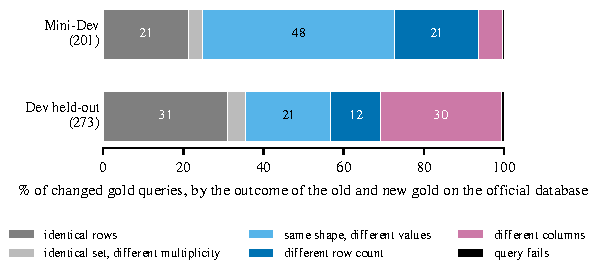
\includegraphics[width=\columnwidth]{figures/fig_execution.pdf}
\caption{Outcome of running each changed gold query and its replacement on the
official database. Grey segments mark changes with an unchanged result set.}
\label{fig:execution}
\end{figure}

A pair with the same result may still be non-equivalent. We re-ran each such pair
on perturbed copies of the tables it references. The perturbations duplicate a
few rows, set referenced columns to \texttt{NULL}, copy extreme sort-key values
into other rows, move dates to a birthday boundary, and delete a random 20\% of
rows, each with three seeds. The perturbations could run on 45 of the 50 hidden
Mini-Dev changes and on 95 of the 97 held-out Dev changes. They separated 14
(31.1\%) and 21 (22.1\%) of them (Table~\ref{tab:mutation}). As a control, we
paired 103 unchanged gold queries with their own parser-regenerated text. The
perturbations ran on 99 of these pairs and separated none.

\begin{table}[t]
\caption{Old and new gold pairs with the same result on the official database,
re-run on perturbed copies of the referenced tables.}
\label{tab:mutation}
\centering
\footnotesize
\begin{tabular}{@{}lrrr@{}}
\toprule
 & Mini-Dev & Held-out Dev & Control \\
\midrule
Pairs tested & 45 & 95 & 99 \\
\midrule
Duplicate rows & 4 & 4 & 0 \\
\texttt{NULL} values & 6 & 8 & 0 \\
Ties at the sort key & 2 & 10 & 0 \\
Birthday boundary & 0 & 1 & 0 \\
Delete 20\% of rows & 10 & 8 & 0 \\
\midrule
Exposed by any & 14 (31.1\%) & 21 (22.1\%) & 0 \\
\bottomrule
\end{tabular}
\end{table}

\section{Case Study: System Rankings}
\label{sec:rankings}

Jin et al.\ ran 16 systems on Dev-100 before and after correction and reported a
Spearman correlation of 0.32 between the two rankings~\cite{jin2026pervasive}.
They describe the correction as the only factor that differs. For each system,
their release contains one prediction file for the original inputs and one for
the corrected inputs. Two facts about these files matter.

First, the authors regenerated the predictions instead of reusing them. The
corrections changed the question in 19 examples and the evidence in 17, so at
most 36 examples had new inputs~\cite{jin2026pervasive}. Yet 12 of the 15
systems we checked differ between the two files on more than 36 examples, 49.5
on average and up to 85. Part of the reported ranking change therefore reflects
run-to-run variation of LLM-based systems, not the corrections. Second, both
released CHESS files are verbatim copies of the gold of the same version, for
all 100 queries. The release thus cannot reproduce the reported change of CHESS
from 62\% to 81\%, the largest in the study. We exclude CHESS.

To isolate the gold, we graded one fixed prediction file against both gold
versions on the official databases (Table~\ref{tab:rank}). Kendall $\tau$~\cite{kendall1938} is 0.80
for the original-input predictions and 0.62 for the corrected-input predictions.
Rankings do change, and one system moves 11 places, but less than the earlier
analysis suggests. With 100 questions, the intervals are wide.

\begin{table}[t]
\caption{Fifteen systems on Dev-100, with one prediction file graded against the
old and the corrected gold. $\tau$ is Kendall's rank correlation with a 95\%
bootstrap interval over questions.}
\label{tab:rank}
\centering
\footnotesize
\begin{tabular}{@{}lrr@{}}
\toprule
Prediction file & original inputs & corrected inputs \\
\midrule
Kendall $\tau$ & 0.80 [0.60, 0.90] & 0.62 [0.33, 0.79] \\
Mean score change (points) & 9.9 & 5.5 \\
Largest score change & 13 & 10 \\
Mean rank change & 1.1 & 2.0 \\
Largest rank change & 4 & 11 \\
\bottomrule
\end{tabular}
\end{table}

State-dependent gold queries add a specific bias. For a top-$k$ tie, a system
that returns every tied row never receives credit. A system that returns a single
row receives credit only if the engine picks the same row as for the gold. For an
empty answer, a system whose query matches nothing receives credit. In the 2025
Dev release, ties, \texttt{NULL} tops, and empty answers cover 33 questions
(2.2\%) before counting fan-outs.

\section{Discussion and Lessons}
\label{sec:discussion}

\textbf{Place in the pipeline.} \sys{} is cheap enough to run while an
annotator writes a gold query, the way a linter runs on code. An annotator who sees
``two rows are tied at the cut'' or ``this count is 641 rows but 88 patients''
can fix the query, reword the question, or confirm the reading on the spot. The
same check can run before every release and in continuous integration for a
benchmark repository. Downstream, its findings help in two ways. Leaderboards can apply a tie-aware scoring rule. Builders of training sets that
reuse gold queries can drop or repair flagged pairs. A model then does not
learn to cut ties arbitrarily or to count join rows.

\textbf{Combining with an LLM reviewer.} \sys{} and SAR-Agent do different jobs.
\sys{} finds a narrow class of problems with proof and no judgment. An LLM
reviewer can judge whether a reading fits the question. In our runs, it rarely noticed that the data make two readings differ at a tie, and a larger model did not change this. A natural combination runs \sys{}
first and gives its evidence to the reviewer or to a person. The reviewer then no
longer judges the whole query. It decides whether the question asks for the 641
rows or the 88 patients.

\textbf{Ratios and averages.} In 10 of the 32 fan-outs in the 2025 release, the
count is part of a percentage or an average. There, the \texttt{DISTINCT}
reading changes one side of the ratio. In six cases it yields a value above
100\%. Such findings show that the count depends on the join, but the second
reading is not a candidate answer. A finer rewrite would apply \texttt{DISTINCT}
consistently to numerator and denominator.

\textbf{More constructs.} The four classes are a start. The engine experiment
exposed a fifth class. A query selects a column that
it neither groups nor aggregates, and SQLite takes the value from an arbitrary
row. The second reading requires the grouping to determine the column
functionally, and execution can test this in the same way. Integer division and
case-sensitive string matching are further candidates whose meaning differs
across engines.

\textbf{Beyond BIRD and SQLite.} The checks need only a parser, the gold query, and
a database the checker can query. The tie and fan-out rewrites use window
functions and \texttt{COUNT(DISTINCT)}, which are standard SQL. Two
parts of our implementation are specific to SQLite. It addresses a row by its
\texttt{rowid}, and it uses \texttt{TEMP} tables that shadow base tables of the
same name. On other engines, a primary key and a session-local copy of the table
serve the same purposes. Benchmarks that host their databases in a cloud
warehouse, such as Spider~2.0-Snow~\cite{lei2025spider2}, permit only the live
checks unless a writable copy is available. The meaning of a \texttt{NULL}-top
finding changes with the engine. A benchmark should
therefore run this check on the engine it uses for scoring.

\subsection{Lessons for benchmark builders}
\label{sec:lessons}

\textbf{Run a state check before release,} on the test and the training
split, and hand its evidence to the reviewers.

\textbf{Decide about ties.} Either write the gold in a tie-complete form, or state
that one row suffices and accept any tied row in scoring. The second option is a
small change to the scorer. Let $G$ be a gold query with a tie finding and $G_c$
its tie-complete reading. The scorer accepts a prediction $P$ if
\begin{align*}
&P(D) = G_c(D), \text{ or}\\
&|P(D)| = |G(D)| \text{ and } P(D) \subseteq G_c(D).
\end{align*}
The first case accepts a system that lists every tied row. The second accepts any
choice of $k$ rows among them. The scorer already has the results that both
cases need, and \sys{} supplies $G_c$.

\textbf{Do not ship questions with empty answers.} Remove them, or mark them as
unanswerable and score them accordingly.

\textbf{Ship witnesses as extra database states.} A latent witness is a one-cell
change on which the gold and its other reading disagree. Test suites add such
states for predictions~\cite{zhong2020test}. Adding them for the gold makes the
benchmark decide between readings instead of leaving the choice to the data.

\textbf{Keep predictions fixed when measuring the effect of corrections.}
Re-running LLM-based systems mixes the effect of the gold with run-to-run
variation. Release the exact predictions that the scorer graded, and check them.

\section{Conclusion and Future Work}
A benchmark checks each gold query on one database state, and a gold query can
return the expected answer there by accident. We defined state-dependent gold
queries and built \sys{}, a deterministic checker that proves each finding by
execution. In three human reviews of the BIRD gold, the review changed the
output of flagged queries 2.3 to 4.1 times as often as that of other queries.
The latest official BIRD Dev release still contains 65 flagged queries. Tie
answers changed when we rebuilt the tables, and LLM reviewers of up to 120B
parameters named few ties without the evidence from \sys{}.

Our results set the agenda for our next steps. (1) \sys{} covers four classes
and 11\% to 20\% of the output changes made by each review. We plan to add
checks for ungrouped columns, integer division, and case-sensitive matching. (2)
All releases come from BIRD and SQLite. We plan to port the checks to other
engines and to benchmarks that publish per-example corrections. (3) Later
releases are a reference, not ground truth, and two annotators judged 37
findings with a wide interval for $\kappa$. We plan a larger annotation with
more annotators and a finer rewrite for ratio queries. (4) Our LLM comparison
uses open models and keyword matching. We plan to run the original o3
configuration and to label its explanations by hand. (5) We measured the effect
on scores with four zero-shot models on one release. An end-to-end study with
published systems and a tie-aware scorer is the natural next experiment. (6) An
LLM assistant produced the codes for the 134 audit corrections. We plan to
re-code them by hand.

\section*{Data and Code Availability}
All gold releases we use are public under CC~BY-SA~4.0. Every artifact needed to
reproduce the results is in a public repository at \url{https://github.com/graphuofm/goldcheck}.
It holds the \sys{} checker, the aligned tables of the five releases, the
baselines, the SAR-Agent re-run and model predictions with all outputs and logs,
the engine and training-split runs, the coding table, both annotators' labels,
and the script behind each number, table, and figure. All models in our
experiments have public weights, and no experiment needs a paid API.

\section*{AI-Generated Content Acknowledgement}
We used an LLM assistant, Claude (Anthropic), to write code, run experiments,
draft and edit text in all sections, and produce the codes in
Table~\ref{tab:taxonomy}. The authors reviewed the code, results, and text and
take responsibility for the content. The 37 findings were labeled by two authors
without AI assistance.

\bibliographystyle{IEEEtran}
\bibliography{references}

\end{document}
